
\section{Selecting Platforms in CLIC}
The key to improving workflow performance with cross-platform computing is mapping tasks to platforms where they can achieve high performance~\cite{sigmodblog}. In CLIC, we take this as a node classification problem and solve it using the Graph Convolutional Network (GCN)~\cite{kipf2016semi}. GCN can not only utilize both operator attributes and topological information to achieve high accuracy but also respond to environmental changes. After pre-training the model, the platform selection is actually a model inference procedure of 
whose execution time is negligible. To our best knowledge, we are the first to adopt GCN in platform selection.

\subsection{Problem Definition}
In CLIC, a logical plan is organized in the form of DAG. We define the DAG as $G = (V, E)$ where $V$ denotes the logical operator and $E$ denotes the operator dependency. Our goal is to find a platform for each logical operator to maximize the performance of a workflow. We consider the most appropriate platform of each operator as the label of the node, which has a strong relationship with the logical plan structure and the workload. Therefore, the goal is transformed into predicting the label of each node in a graph structure which is a typical node classification problem~\cite{bhagat2011node}. 

\subsection{Graph Convolutional Network}
Graph Convolutional Network is a convolutional neural network that can be directly applied to graphs. It stacks layers of learned first-order spectral filters, which are followed by an activation function to learn graph representations~\cite{wu2019simplifying}. 

GCN relies on a graph convolution layer to capture topological information. The process is shown at the top of Figure \ref{fig:gcn}. It first traverses each node in the graph and samples K (a hyperparameter) neighboring nodes to form a subgraph. If the node has less than K first-level neighbors, then it adds second-level neighbors. After that, it normalizes all subgraphs to a $K \times |V|$ matrix and applies the convolutional kernel~\cite{dai2017deformable} to learn the joint information. Finally, it passes the matrix through an activation function such as ReLU~\cite{hahnloser2000digital}. The output is a dense matrix with each column representing the node embedding that can be later used to predict the label. The whole convolution process can be formulated as Equation \ref{eq:graph-conv} where $\frac{1}{\omega}$ is the normalization term with $\omega$ equaling to the cardinality of the neighbor set, i.e., the K in this case. $B(v^i) = {v^j | d(v^i, v^j) \leq D }$ is the neighbor set of vertices $v^i$. $d(v^i, v^j)$ denotes the shortest path connecting $v^i$ and $v^j$, and $\sigma$ is the activation function.


\begin{equation}
    v^{i(l+1)} = \sigma (\frac{1}{\omega} \sum_{ v^{j(l)} \in B(v^{i(l)}) } p(v^{i(l)}, v^{j(l)}) w(v^{i(l)}, v^{j(l)})  )  )
    \label{eq:graph-conv}
\end{equation}

\begin{figure}
  \centering
  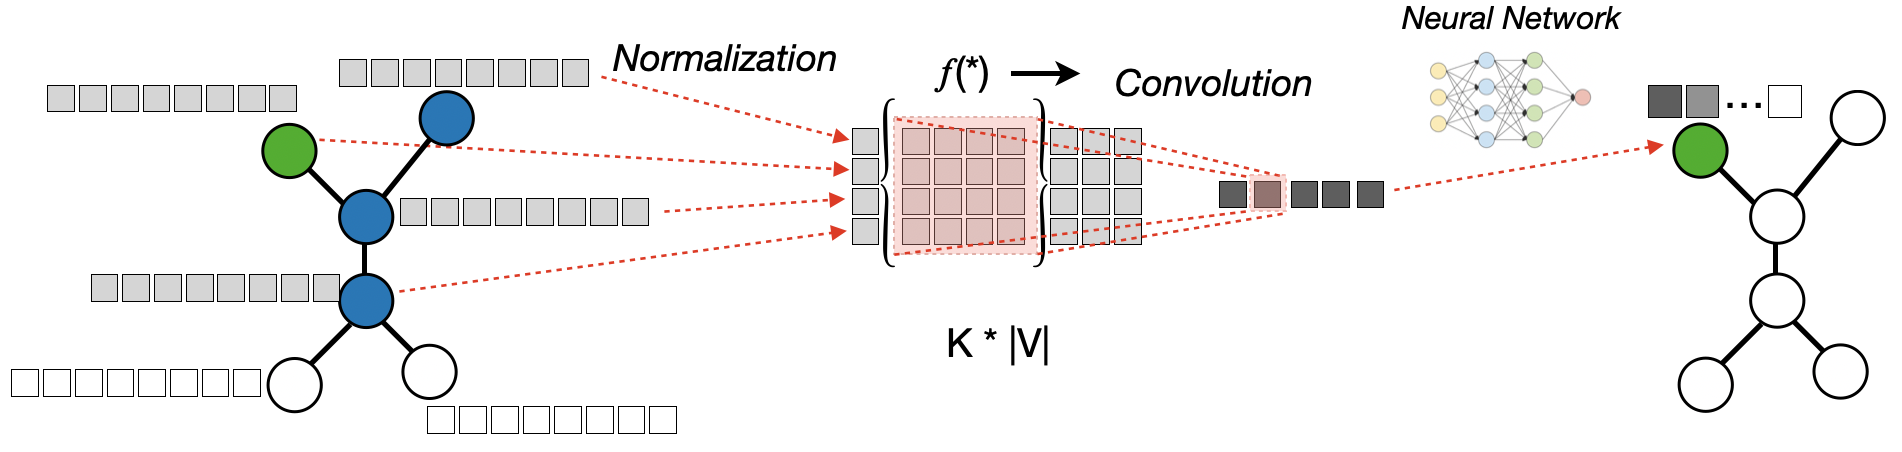
\includegraphics[width=0.9\linewidth]{figures/gcn.pdf}
  \caption{Selecting platforms with GCN}
  \label{fig:gcn}
\end{figure}

\subsection{GCN implementation in CLIC}
The complete GCN structure in CLIC is shown in Figure \ref{fig:gcn}. We add a dropout layer~\cite{srivastava2014dropout} right after the graph convolutional layer as it is a common way to help prevent overfitting~\cite{baldi2013understanding}. In order to classify nodes based on their embedding, we add a fully-connected layer at the end of GCN. The output of this layer is the confidence vector of each operator, which indicates the probability of each platform for achieving the highest overall performance. Moreover, we put a binary mask on each final confidence vector in case the predicated platform doesn’t support that operator.

The input of the GCN is the logical plan. We assign an initial feature vector to each operator that consists of its own attributes and global environmental settings. The attributes include the operator’s cardinality and the one-hot encoding of operator id used to distinguish each operator. Hardware environments and computing platform configurations are flattened into a long and sparse vector as global environmental settings and embedded into each operator’s feature vector. 

Although the GCN can theoretically overcome the selection problem, its effectiveness highly relies on sufficient training data, i.e., large amounts of logical plans and its operators’ label. Therefore, we synthetic the dataset following the pattern in TDGen~\cite{kaoudi2020ml} which including four steps: 1) randomly generating synthetic logical plans of different shapes and sizes; 2) enumerating all possible physical plans for a logical plan and using a heuristic pruning operation~\cite{kaoudi2020ml} to prune the search space; 3) executing each pruned physical plan to find the one with the highest performance and labeling logical operators as the corresponding platforms in the best physical plan; 4) repeating the third step with different workloads and using the interpolation technique to enrich the dataset. By always choosing the best physical plan as a training data label, the data transmission cost can be implicitly learned by GCN.

\begin{figure*}
    \centering
    \subfigure[Word2Vec]{
        \label{fig:single-word2vec}
        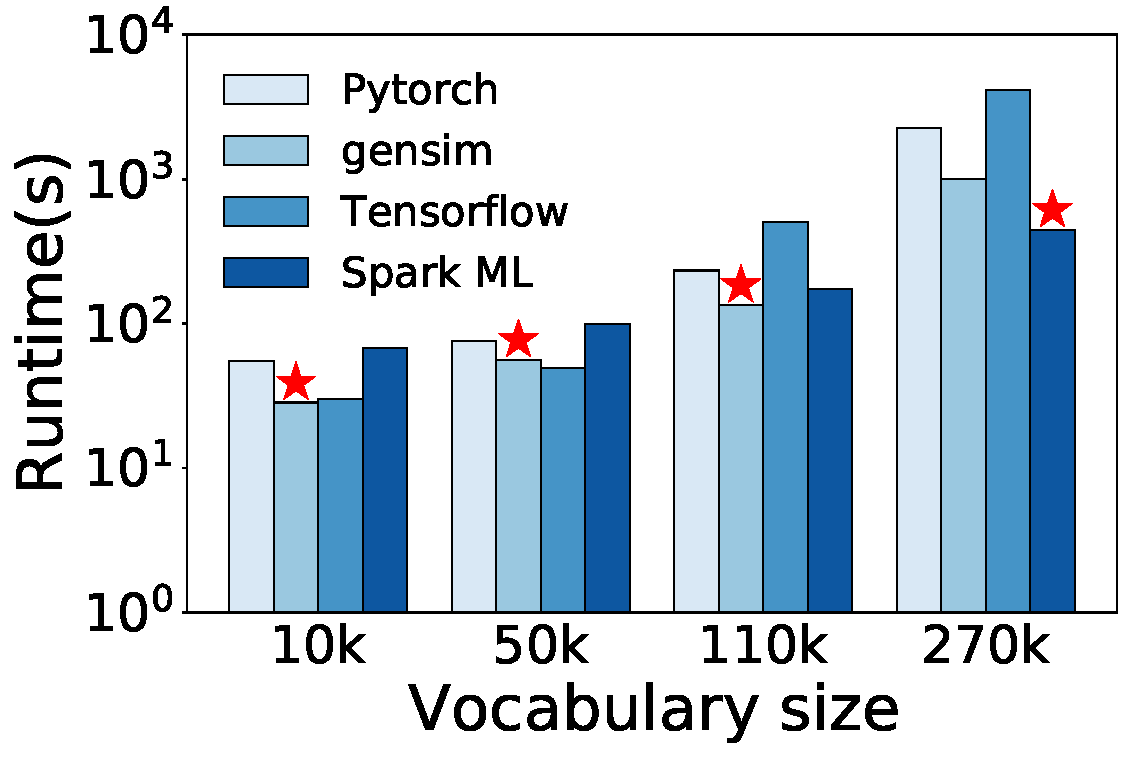
\includegraphics[width=0.23\textwidth]{figures/chp6-word2vec.pdf}
    } 
    \subfigure[PCA]{
    \label{fig:single-PCA}
        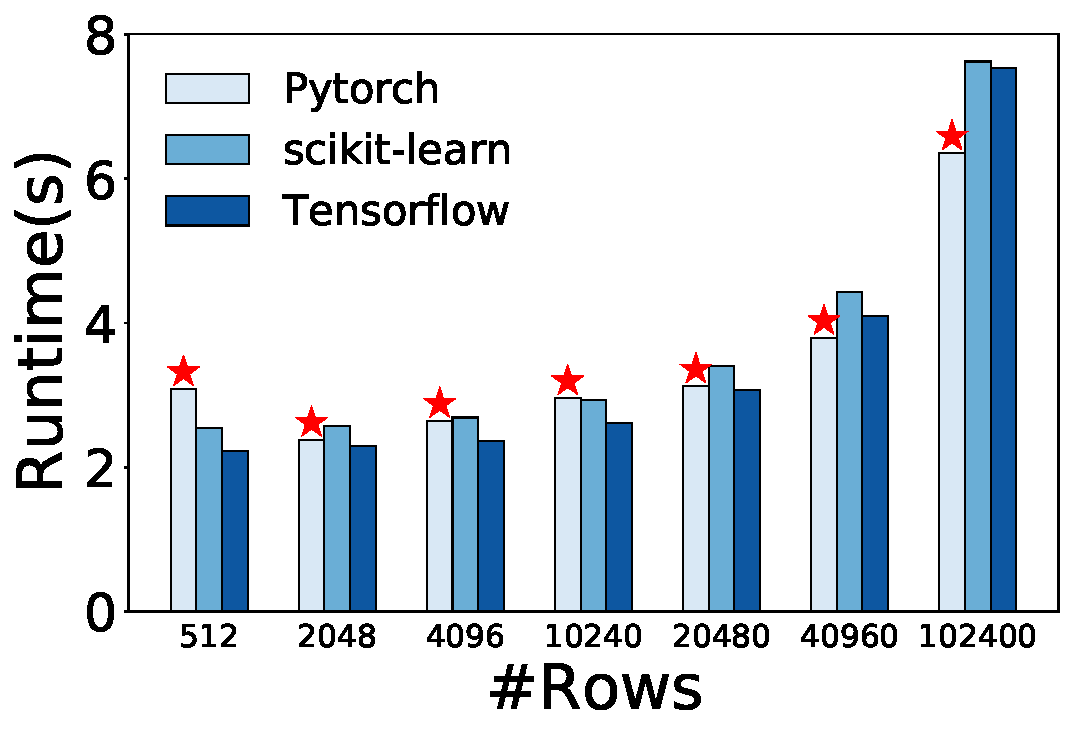
\includegraphics[width=0.23\textwidth]{figures/chp6-PCA.pdf}
    } 
    \subfigure[PageRank]{
    \label{fig:single-PR}
        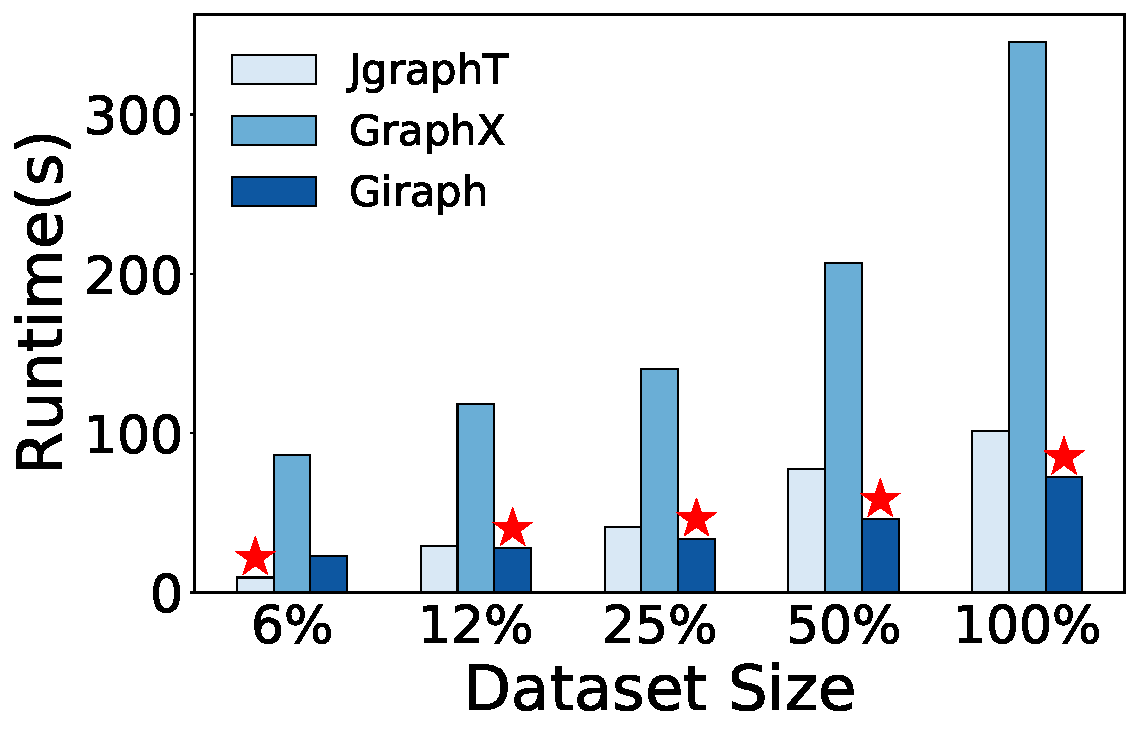
\includegraphics[width=0.23\textwidth]{figures/chp6-PR.pdf}
    }
    \subfigure[WordCount]{
    \label{fig:single-wc}
        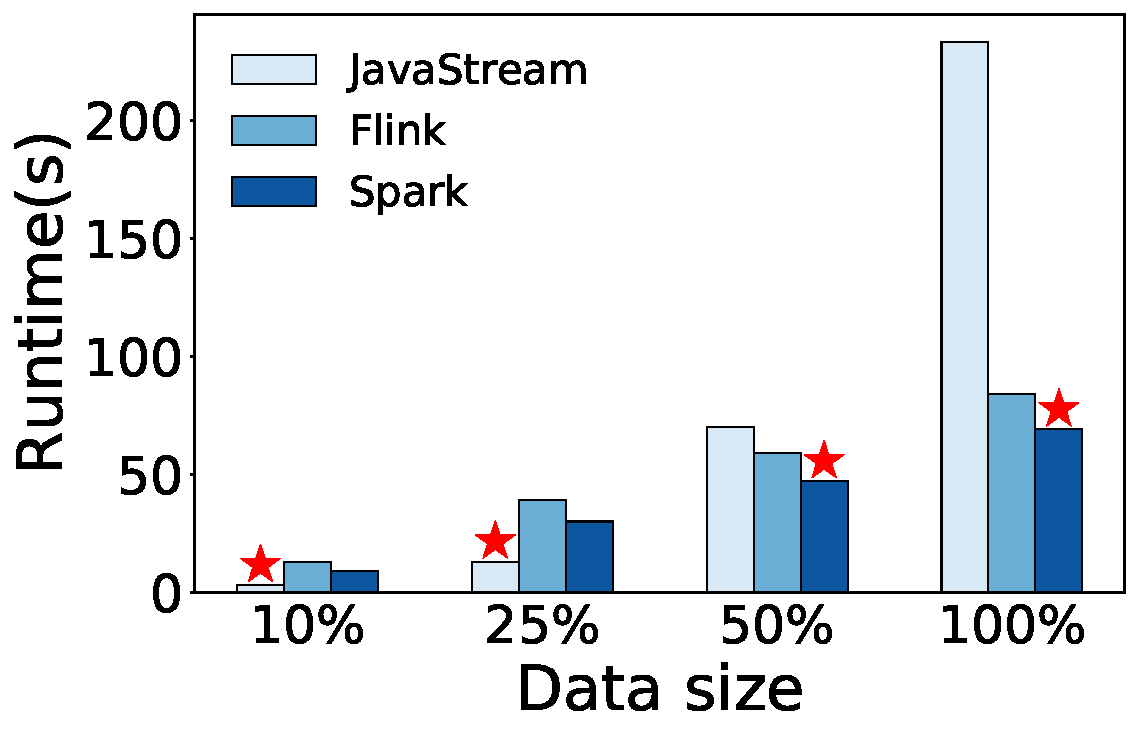
\includegraphics[width=0.23\textwidth]{figures/chp6-wordcount.pdf}
    }
    \caption{Single operator selection}
    \label{fig:single-opt-selection}
\end{figure*}